\documentclass[11pt]{beamer}
\usepackage[utf8]{inputenc}
\usepackage[T1]{fontenc}
\usepackage{amsmath}
\usepackage{amssymb}
\usepackage{graphicx}
\usepackage[english]{babel}
\usepackage{url}
\usepackage{hyperref}
\usepackage{listings}
\usepackage{textcomp}
\usepackage{accsupp}
\usepackage{attachfile}
\usepackage{verbatim}
\usepackage[misc]{ifsym}
\usepackage[super]{nth}
\usepackage{dirtree}

% color def
\usepackage{color}
\definecolor{darkred}{rgb}{0.6,0.0,0.0}
\definecolor{darkgreen}{rgb}{0,0.50,0}
\definecolor{lightblue}{rgb}{0.0,0.42,0.91}
\definecolor{orange}{rgb}{0.99,0.48,0.13}
\definecolor{grass}{rgb}{0.18,0.80,0.18}
\definecolor{pink}{rgb}{0.97,0.15,0.45}

\usepackage{tikz}
\usetikzlibrary{shapes.multipart}
\usetikzlibrary {shapes.misc} 
\usetikzlibrary{shadows.blur}
\usetikzlibrary{positioning}
\usetikzlibrary{arrows}
\usetikzlibrary{matrix}
\tikzset{
stack_item/.style={rounded rectangle, rounded rectangle arc length=90,draw, anchor=center, fill=white, minimum width=1cm},
bar/.style={rounded rectangle, minimum width=1.5cm, fill=black, blur shadow={shadow blur steps=5,shadow blur extra rounding=1.3pt}},
message/.style={rectangle, fill=white, color=white, text=black},
bowling_pin/.style={circle, draw, line width=0.6mm, color=red, text=black, minimum width=8mm},
empty/.style={circle, draw, line width=0.6mm, color=white, text=black, minimum width=8mm},
table_cell/.style={rectangle, draw, color=black, text=black, minimum size=12mm}
}

% listings
\usepackage{listings}

% General Setting of listings
\lstset{
	language=Python,
	tabsize=4,
	aboveskip=1em,
	breaklines=true,
	abovecaptionskip=-6pt,
	captionpos=b,
	escapeinside={\%*}{*)},
	frame=single,
	numbers=left,
	numbersep=8pt,
	numberstyle=\tiny,
	morekeywords=[1]{,as,assert,nonlocal,with,yield,self,True,False,None,} % Python builtin
	morekeywords=[2]{,__init__,__add__,__mul__,__div__,__sub__,__call__,__getitem__,__setitem__,__eq__,__ne__,__nonzero__,__rmul__,__radd__,__repr__,__str__,__get__,__truediv__,__pow__,__name__,__future__,__all__,}, % magic methods
	morekeywords=[3]{,object,type,isinstance,copy,deepcopy,zip,enumerate,reversed,list,set,len,dict,tuple,range,xrange,execfile,real,imag,reduce,str,repr,}, % common functions
	morekeywords=[4]{,Exception,NameError,IndexError,SyntaxError,TypeError,ValueError,OverflowError,ZeroDivisionError,}, % errors
	morekeywords=[5]{,ode,fsolve,sqrt,exp,sin,cos,arctan,arctan2,arccos,pi, array,norm,solve,dot,arange,isscalar,max,sum,flatten,shape,reshape,find,any,all,abs,plot,linspace,legend,quad,polyval,polyfit,hstack,concatenate,vstack,column_stack,empty,zeros,ones,rand,vander,grid,pcolor,eig,eigs,eigvals,svd,qr,tan,det,logspace,roll,min,mean,cumsum,cumprod,diff,vectorize,lstsq,cla,eye,xlabel,ylabel,squeeze,}, % numpy / math
	deletekeywords=[2]{next,set},
	deletekeywords=[3]{next,set},
	basicstyle=\ttfamily,
	backgroundcolor=\color{white},
	commentstyle=\color{darkgreen},
	keywordstyle=\color{blue}\bfseries\itshape,
	keywordstyle=[2]\color{blue}\bfseries,
	keywordstyle=[3]\color{grass},
	keywordstyle=[4]\color{red},
	keywordstyle=[5]\color{orange},
	stringstyle=\color{darkred},
	emphstyle=\color{pink}\underbar,
	morestring=[d]{"},
	showstringspaces=false,
	upquote=true,
}

\usetheme{Darmstadt}
\setbeamertemplate{navigation symbols}{}
\setbeamertemplate{footline}{
	\begin{beamercolorbox}[ht=3ex,leftskip=1.4cm,rightskip=.3cm]{author in head/foot}
		\hfill \insertframenumber
		\vspace*{0.07cm}
	\end{beamercolorbox}
} 

\title{Ejemplo calculadora postfix}
\titlegraphic{
\includegraphics[width=3cm]{img/UPNA}}
%\date[]{2024-2025}
\date{}
\author{Estructura de Datos}
\subject{Estructura de Datos}

\begin{document}
\begin{frame}[plain]
	\maketitle
\end{frame}

\begin{frame}
\begin{center}
\scalebox{1.5}{
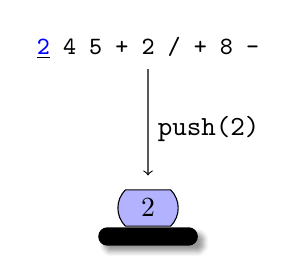
\begin{tikzpicture}
    \node[message] (formula_1) {\small\texttt{{\underline{\color{blue}2}} 4 5 + 2 / + 8 -}};
    \node[bar] (base_1) [below=2cm of formula_1] {};
    \node[stack_item, fill=blue!30] (1_1) [above=0 of base_1] {2};
    \draw[->, shorten >=5pt] (formula_1) -- (1_1) node[midway, right] {\texttt{push(2)}};
\end{tikzpicture}
}
\end{center}
\end{frame}

\begin{frame}
\begin{center}
\scalebox{1.5}{
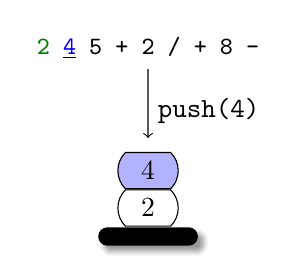
\begin{tikzpicture}
    \node[message] (formula_2) {\small\texttt{{\color{darkgreen}2} {\underline{\color{blue}4}} 5 + 2 / + 8 -}};
    \node[bar] (base_2) [below=2cm of formula_2] {};
    \node[stack_item] (1_2) [above=0 of base_2] {2};
    \node[stack_item, fill=blue!30] (2_2) [above=0 of 1_2] {4};
    \draw[->, shorten >=5pt] (formula_2) -- (2_2) node[midway, right] {\texttt{push(4)}};
\end{tikzpicture}
}
\end{center}
\end{frame}

\begin{frame}
\begin{center}
\scalebox{1.5}{
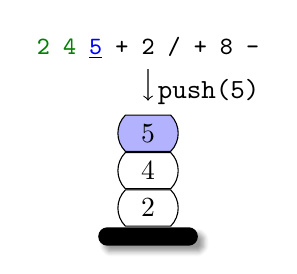
\begin{tikzpicture}
    \node[message] (formula_3) {\small\texttt{{\color{darkgreen}2 4} {\underline{\color{blue}5}} + 2 / + 8 -}};
    \node[bar] (base_3) [below=2cm of formula_3] {};
    \node[stack_item] (1_3) [above=0 of base_3] {2};
    \node[stack_item] (2_3) [above=0 of 1_3] {4};
    \node[stack_item, fill=blue!30] (3_3) [above=0 of 2_3] {5};
    \draw[->, shorten >=5pt] (formula_3) -- (3_3) node[midway, right] {\texttt{push(5)}};
\end{tikzpicture}
}
\end{center}
\end{frame}

\begin{frame}
\begin{center}
\scalebox{1.5}{
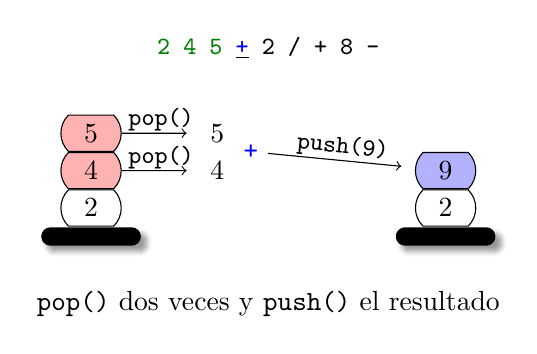
\begin{tikzpicture}
    \node[message] (formula_4) {\small\texttt{{\color{darkgreen}2 4 5} {\underline{\color{blue}+}} 2 / + 8 -}};
    \node[bar] (base_4) [below left=2cm and 0.2cm of formula_4] {};
    \node[stack_item] (1_4) [above=0 of base_4] {2};
    \node[stack_item, fill=red!30] (2_4) [above=0 of 1_4] {4};
    \node[stack_item, fill=red!30] (3_4) [above=0 of 2_4] {5};
    
    \node[message] (m_3_4) [right=of 3_4] {5};
    \node[message] (m_2_4) [right=of 2_4] {4};
    \draw[->, shorten >=5pt] (3_4) -- (m_3_4) node[midway, above=-0.1cm] {\small\texttt{pop()}};
    \draw[->, shorten >=5pt] (2_4) -- (m_2_4) node[midway, above=-0.1cm] {\small\texttt{pop()}};
    \node[message] (m_plus_4) [below right=-2.2mm and 0mm of m_3_4] {\texttt{\color{blue}+}};
    
    \node[message] (message_4) [below=2.7cm of formula_4] {\texttt{pop()} dos veces y \texttt{push()} el resultado};
    
    \node[bar] (base_4_1) [below right=2cm and 0.2cm of formula_4] {};
    \node[stack_item] (1_4_1) [above=0 of base_4_1] {2};
    \node[stack_item, fill=blue!30] (2_4_1) [above=0 of 1_4_1] {9};
    \draw[->, shorten >=5pt] (m_plus_4) -- (2_4_1) node[sloped, midway, above=-0.1cm] {\small\texttt{push(9)}};
\end{tikzpicture}
}
\end{center}
\end{frame}


\begin{frame}
\begin{center}
\scalebox{1.5}{
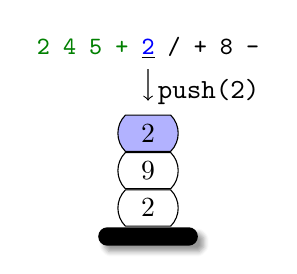
\begin{tikzpicture}
    \node[message] (formula_5) {\small\texttt{{\color{darkgreen}2 4 5 +} {\underline{\color{blue}2}} / + 8 -}};
    \node[bar] (base_5) [below=2cm of formula_5] {};
    \node[stack_item] (1_5) [above=0 of base_5] {2};
    \node[stack_item] (2_5) [above=0 of 1_5] {9};
    \node[stack_item, fill=blue!30] (3_5) [above=0 of 2_5] {2};
    \draw[->, shorten >=5pt] (formula_5) -- (3_5) node[midway, right] {\texttt{push(2)}};
\end{tikzpicture}
}
\end{center}
\end{frame}

\begin{frame}
\begin{center}
\scalebox{1.5}{
\begin{tikzpicture}
    \node[message] (formula_6) {\small\texttt{{\color{darkgreen}2 4 5 + 2} {\underline{\color{blue}/}} + 8 -}};
    \node[bar] (base_6) [below left=2cm and 0.2cm of formula_6] {};
    \node[stack_item] (1_6) [above=0 of base_6] {2};
    \node[stack_item, fill=red!30] (2_6) [above=0 of 1_6] {9};
    \node[stack_item, fill=red!30] (3_6) [above=0 of 2_6] {2};
    
    \node[message] (m_3_6) [right=of 3_4] {2};
    \node[message] (m_2_6) [right=of 2_4] {9};
    \draw[->, shorten >=5pt] (3_6) -- (m_3_6) node[midway, above=-0.1cm] {\small\texttt{pop()}};
    \draw[->, shorten >=5pt] (2_6) -- (m_2_6) node[midway, above=-0.1cm] {\small\texttt{pop()}};
    \node[message] (m_div_6) [below right=-2.2mm and 0mm of m_3_6] {\texttt{\color{blue}/}};
    
    \node[message] (message_6) [below=2.7cm of formula_6] {\underline{\textbf{Observa el orden de operaciones: \texttt{9/2}}}};
    
    \node[bar] (base_6_1) [below right=2cm and 0.2cm of formula_6] {};
    \node[stack_item] (1_6_1) [above=0 of base_6_1] {2};
    \node[stack_item, fill=blue!30] (2_6_1) [above=0 of 1_6_1] {4.5};
    \draw[->, shorten >=5pt] (m_div_6) -- (2_6_1) node[sloped, midway, above=-0.1cm] {\small\texttt{push(4.5)}};
\end{tikzpicture}
}
\end{center}
\end{frame}

\begin{frame}
\begin{center}
\scalebox{1.5}{
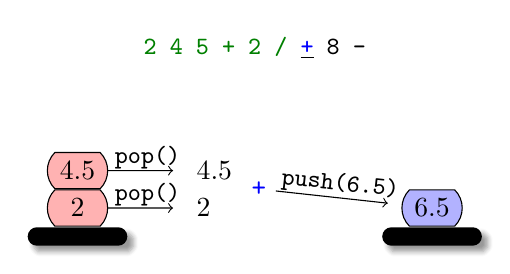
\begin{tikzpicture}
    \node[message] (formula_7) {\small\texttt{{\color{darkgreen}2 4 5 + 2 /} {\underline{\color{blue}+}} 8 -}};
    \node[bar] (base_7) [below left=2cm and 0.2cm of formula_7] {};
    \node[stack_item, fill=red!30] (1_7) [above=0 of base_7] {2};
    \node[stack_item, fill=red!30] (2_7) [above=0 of 1_7] {4.5};
    
    \node[message] (m_2_7) [right=of 2_7] {4.5};
    \node[message] (m_1_7) [right=of 1_7] {2};
    \draw[->, shorten >=5pt] (2_7) -- (m_2_7) node[midway, above=-0.1cm] {\small\texttt{pop()}};
    \draw[->, shorten >=5pt] (1_7) -- (m_1_7) node[midway, above=-0.1cm] {\small\texttt{pop()}};
    \node[message] (m_plus_7) [below right=-2.2mm and 0mm of m_2_7] {\texttt{\color{blue}+}};
    
    \node[bar] (base_7_1) [below right=2cm and 0.2cm of formula_7] {};
    \node[stack_item, fill=blue!30] (1_7_1) [above=0 of base_7_1] {6.5};
    \draw[->, shorten >=5pt] (m_plus_7) -- (1_7_1) node[sloped, midway, above=-0.1cm] {\small\texttt{push(6.5)}};
\end{tikzpicture}
}
\end{center}
\end{frame}

\begin{frame}
\begin{center}
\scalebox{1.5}{
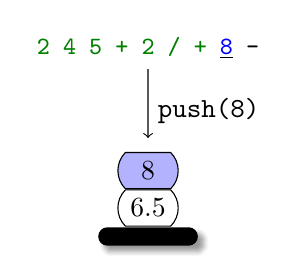
\begin{tikzpicture}
    \node[message] (formula_8) {\small\texttt{{\color{darkgreen}2 4 5 + 2 / +} {\underline{\color{blue}8}} -}};
    \node[bar] (base_8) [below=2cm of formula_8] {};
    \node[stack_item] (1_8) [above=0 of base_8] {6.5};
    \node[stack_item, fill=blue!30] (2_8) [above=0 of 1_8] {8};
    \draw[->, shorten >=5pt] (formula_8) -- (2_8) node[midway, right] {\texttt{push(8)}};
\end{tikzpicture}
}
\end{center}
\end{frame}


\begin{frame}
\begin{center}
\scalebox{1.5}{
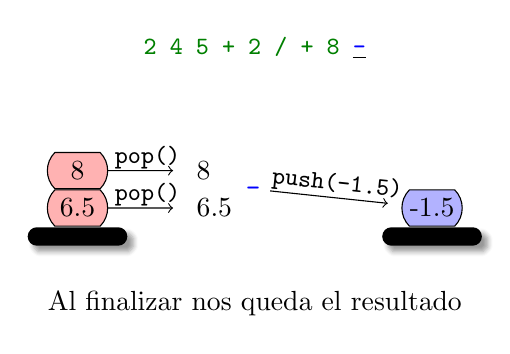
\begin{tikzpicture}
    \node[message] (formula_9) {\small\texttt{{\color{darkgreen}2 4 5 + 2 / + 8} {\underline{\color{blue}-}}}};
    \node[bar] (base_9) [below left=2cm and 0.2cm of formula_9] {};
    \node[stack_item, fill=red!30] (1_9) [above=0 of base_9] {6.5};
    \node[stack_item, fill=red!30] (2_9) [above=0 of 1_9] {8};
    
    \node[message] (m_2_9) [right=of 2_9] {8};
    \node[message] (m_1_9) [right=of 1_9] {6.5};
    \draw[->, shorten >=5pt] (2_9) -- (m_2_9) node[midway, above=-0.1cm] {\small\texttt{pop()}};
    \draw[->, shorten >=5pt] (1_9) -- (m_1_9) node[midway, above=-0.1cm] {\small\texttt{pop()}};
    \node[message] (m_minus_9) [below right=-2.2mm and 2mm of m_2_9] {\texttt{\color{blue}-}};
    
    \node[bar] (base_9_1) [below right=2cm and 0.2cm of formula_9] {};
    \node[stack_item, fill=blue!30] (1_9_1) [above=0 of base_9_1] {-1.5};
    \draw[->, shorten >=5pt] (m_minus_9) -- (1_9_1) node[sloped, midway, above=-0.1cm] {\small\texttt{push(-1.5)}};
    
    \node[message] (message_9) [below=2.7cm of formula_9] {Al finalizar nos queda el resultado};
\end{tikzpicture}
}
\end{center}
\end{frame}


\end{document}